%%%%%%%%%%%%%%%%%%%%%%%%%%%%%%%%%%%%%%%%%%%%%%%%%%%%%%%%%%%%%%%%%%%%%%
% LaTeX Template: Two Column Colour Article
%
% Source: http://www.howtotex.com/
% Feel free to distribute this template, but please keep the
% referal to howtotex.com.
% Date: Feb 2011
% 

%%% Preamble
\documentclass[	DIV=calc,%
paper=a4,%
fontsize=11pt,%
twocolumn]{scrartcl} % KOMA-article class

\usepackage{lipsum}	% Package to create dummy text
\usepackage[english]{babel}	% English language/hyphenation
\usepackage[protrusion=true,expansion=true]{microtype}	% Better typography
\usepackage{amsmath,amsfonts,amsthm} % Math packages
\usepackage[pdftex]{graphicx} % Enable pdflatex
\usepackage{wrapfig} % enable figure wrapping
\usepackage[svgnames]{xcolor} % Enabling colors by their 'svgnames'
\usepackage[hang, small,labelfont=bf,up,textfont=it,up]{caption} % Custom captions under/above floats
\usepackage{epstopdf} % Converts .eps to .pdf
\usepackage{subfig}	% Subfigures
\usepackage{booktabs} % Nicer tables
\usepackage{fix-cm}	% Custom fontsizes
\usepackage{booktabs} % prof. looking tables (www.en.wikibooks.org/wiki/LaTeX/Tables#Professional_tables)
\usepackage{tikz}
\usepackage{amsmath}
\usetikzlibrary{quotes,angles}
\usepackage{mathtools}
\usepackage{tkz-euclide}
\usetikzlibrary{decorations.pathreplacing}
\usepackage{svg}
\usepackage{tikz-3dplot}

%%% Custom sectioning (sectsty package)
\usepackage{sectsty} % Custom sectioning (see below)
\allsectionsfont{%		% Change font of al section commands
	\usefont{OT1}{phv}{b}{n}%	% bch-b-n: CharterBT-Bold font
}

\sectionfont{%		% Change font of \section command
	\usefont{OT1}{phv}{b}{n}%	% bch-b-n: CharterBT-Bold font
}


%%% Headers and footers
\usepackage{fancyhdr} % Needed to define custom headers/footers
\pagestyle{fancy} % Enabling the custom headers/footers
\usepackage{lastpage}	

% Header (empty)
\lhead{}
\chead{}
\rhead{\today}
% Footer (you may change this to your own needs)
\lfoot{\footnotesize \texttt{Math Notes for ML} \textbullet ~ Bhargav}
\cfoot{}
\rfoot{\footnotesize page \thepage\ of \pageref{LastPage}}	% "Page 1 of 2"
\renewcommand{\headrulewidth}{0.0pt}
\renewcommand{\footrulewidth}{0.4pt}
\newcommand{\hformbar}[1]{\vspace{5pt}\hrule\vspace{10pt}} % creates a horizontal bar to separate formulae better; space adaptions can be made centrally here


%%% Creating an initial of the very first character of the content
\usepackage{lettrine}
\newcommand{\initial}[1]{%
	\lettrine[lines=3,lhang=0.3,nindent=0em]{
		\color{DarkGoldenrod}
		{\textsf{#1}}}{}}

%%% Title, author and date metadata
\usepackage{titling} % For custom titles

\newcommand{\HorRule}{\color{DarkGoldenrod}%	% Creating a horizontal rule
	\rule{\linewidth}{1pt}%
}

\pretitle{\vspace{-30pt} \begin{flushleft} \HorRule 
		\fontsize{20}{20} \usefont{OT1}{phv}{b}{n} \color{DarkRed} \selectfont 
	}
	\title{Linear Algebra + Stats + Probability Notes} % Title of your article goes here
	\posttitle{\par\end{flushleft}\vskip 0.5em}

\preauthor{\begin{flushleft}\large \lineskip 0.5em \usefont{OT1}{phv}{b}{sl} \color{DarkRed}}
	\author{Bhargav} % Author name goes here
	\postauthor{\footnotesize \usefont{OT1}{phv}{m}{sl} \color{Black} \hspace{5pt} github.com/brpy/ml-notes \par\end{flushleft}\HorRule}

\date{\today} % No date

%%% wws: create a non-indented formula name
\newcommand{\formdesc}[1]{\noindent\textbf{#1}}

% A 2x2 shape matrix
\newcommand{\tctmat}[4]{\begin{bmatrix}
		$#1$ & $#2$\\
		$#3$ & $#4$
\end{bmatrix}}

% A 2x1 shape matrix
\newcommand{\tcomat}[2]{\begin{bmatrix}
		$#1$\\
		$#2$
\end{bmatrix}}

% A 3x3 shape matrix
\newcommand{\thcthmat}[9]{\begin{bmatrix}
		$#1$ & $#2$ & $#3$\\
		$#4$ & $#5$ & $#6$\\
		$#7$ & $#8$ & $#9$
\end{bmatrix}}

% A 3x1 shape matrix
\newcommand{\thcomat}[3]{\begin{bmatrix}
		$#1$\\
		$#2$\\
		$#3$
\end{bmatrix}}

\DeclareUnicodeCharacter{03C6}{$\phi$ }
\DeclareUnicodeCharacter{03C3}{$\sigma$ }
\DeclareUnicodeCharacter{03BC}{$\mu$ }
\DeclareUnicodeCharacter{2212}{$-$}
\DeclareUnicodeCharacter{03A6}{$\Phi$ }
\DeclareUnicodeCharacter{2248}{$\approx$ }

%%% Begin document -----------------------------------------------------------------
\begin{document}
	\maketitle
	\thispagestyle{fancy} 	% Enabling the custom headers/footers for the first page 
	% The first character should be within \initial{}
	\section{Linear Algebra}
	
	\textbf{The following notes is primarily made for my revision. I might have skipped some topics that seemed obvious to me. I do not guarantee factual correctness of the notes. If you feel there are any errors, open a github issue/pr. Notes material is collected from various sources. Image credits are given in tex document and in src.csv}
	
	\hspace{10pt}

\hformbar
\formdesc{Vectors:}

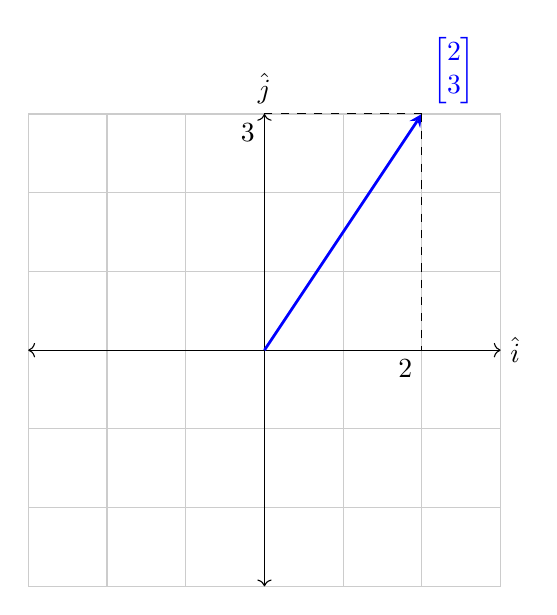
\begin{tikzpicture}
	\draw[thin,gray!40] (-3,-3) grid (3,3);
	\draw[<->] (-3,0)--(3,0) node[right]{$\hat{i}$};
	\draw[<->] (0,-3)--(0,3) node[above]{$\hat{j}$};
	\draw[line width=1pt,blue,-stealth](0,0)--(2,3) node[anchor=south west]{$\boldsymbol{\tcomat{2}{3}}$};
	\draw [dashed] (2,3)--(2,0) node[anchor=north east]{${2}$};
	\draw [dashed] (2,3)--(0,3) node[anchor=north east]{${3}$};
\end{tikzpicture}
\begin{itemize}
	\item This vector is represented as $2\hat{i} + 3\hat{j}$ where $\hat{i}$ and $\hat{j}$ are unit vectors perpendicular to each other also known as basis vectors (in 2d).
	\item It is also represented as a column matrix $\tcomat{2}{3}$
	\item A vector is represented by its length and direction wrto. basis vectors $\hat{i}$, $\hat{j}$.
	\item A vector can be freely moved without changing its length and the direction it is pointing to.
	\item So any vector in space can be represented using a linear combination of $\hat{i}$, $\hat{j}$ by moving the starting point to origin.
\end{itemize}

\hformbar
\formdesc{Adding 2 Vectors:}

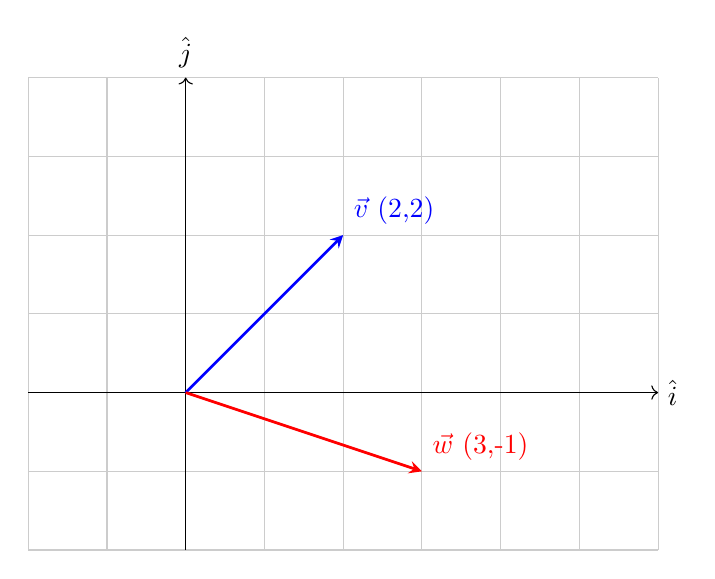
\begin{tikzpicture}
	\draw[thin,gray!40] (-2,-2) grid (6,4);
	\draw[.->] (-2,0)--(6,0) node[right]{$\hat{i}$};
	\draw[.->] (0,-2)--(0,4) node[above]{$\hat{j}$};
	\draw[line width=1pt,blue,-stealth](0,0)--(2,2) node[anchor=south west]{$\vec{v}$	(2,2)};
	\draw[line width=1pt,red,-stealth](0,0)--(3,-1) node[anchor=south west]{$\vec{w}$	(3,-1)};
\end{tikzpicture}

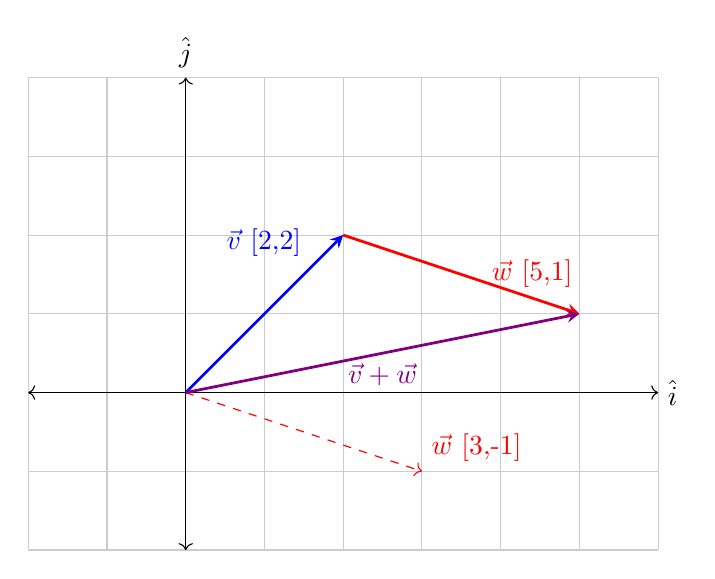
\begin{tikzpicture}
	\draw[thin,gray!40] (-2,-2) grid (6,4);
	\draw[<->] (-2,0)--(6,0) node[right]{$\hat{i}$};
	\draw[<->] (0,-2)--(0,4) node[above]{$\hat{j}$};
	\draw[line width=1pt,blue,-stealth](0,0)--(2,2) node[anchor=south east, pos=0.8]{$\vec{v}$	[2,2]};
	\draw[red, dashed, ->](0,0)--(3,-1) node[anchor=south west]{$\vec{w}$	[3,-1]};
	\draw[line width=1pt,red,-stealth](2,2)--(5,1) node[anchor=south, pos=0.8]{$\vec{w}$	 [5,1]};
	\draw[line width=1pt,violet,-stealth](0,0)--(5,1) node[anchor=north, pos=0.5]{$\vec{v} + \vec{w}$};
\end{tikzpicture}
This is also known as Triangular law of vector addition.




\begin{itemize}
	\item Can also be interpreted as,
	
	
	$\boldsymbol{\tcomat{5}{1}}$ = $\boldsymbol{\tcomat{2}{2}}$ + $\boldsymbol{\tcomat{3}{-1}}$
	\item The vector $\vec{w}$ is moved along $\vec{v}$ such that the starting point of $\vec{w}$ meets the end point of $\vec{v}$
	\item Both $\vec{v}$ and $\vec{w}$ direction and lengths remain unchanged.

\end{itemize}

\hformbar
\formdesc{Scaling:}

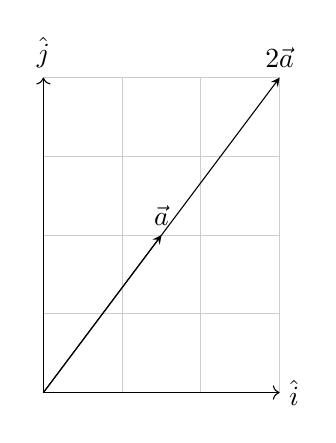
\begin{tikzpicture}
	\draw[thin,gray!40] (0,0) grid (3,4);
	\draw[.-> ] (0,0)--(3,0) node[right]{$\hat{i}$};
	\draw[.->] (0,0)--(0,4) node[above]{$\hat{j}$};
	\draw[.->,-stealth] (0,0)--(1.5,2)  coordinate (a)  node[above]{$\vec{a}$};
	\draw[.->,-stealth] (0,0)--(3,4) node[above]{$2\vec{a}$};
\end{tikzpicture}

\begin{itemize}
	\item 2 \emph{scales} the vector $\vec{a}$.
	So, 2 is a Scalar.
	\item Similarly basis vectors $\hat{i}$ and $\hat{j}$ can be scaled to represent any vector in 2d plane.
	
\end{itemize}

\hformbar
\formdesc{Span:}

\begin{itemize}

\item $a\vec{v}+b\vec{w}$ $\implies$ Linear combination of $\vec{v}$, $\vec{w}$

\item Set of all vectors of linear combination of $\vec{v}$, $\vec{w}$ ; $a\vec{v}+b\vec{w}$ is called \textbf{span}.


\item For most vectors span consists of all points on the plane.

\item If $\vec{v}$, $\vec{w}$ lie on same line, span is a line passin through origin.

\item If both $\vec{v}$, $\vec{w}$ are zero, span is zero.
\end{itemize}

\hformbar
\formdesc{Linear (in)dependent:}
\begin{itemize}
	\item If one vector can be represented as a linear combination of other, then the vectors are linearly dependent.
	\item A linearly dependent vector doesn't add to span of a vector.
	\item If one vector adds a dimension to a span of a vector, they are linearly independent.
\end{itemize}

\hformbar
\formdesc{Transformation:}
\begin{itemize}
	\item Takes a vector and gives a output vector.
\end{itemize}

\hformbar
\formdesc{Linear Transformation:}

The conditions for the tranformation to be linear are:

\begin{itemize}
	\item All lines must remain lines.
	\item Origin must be remain inplace.
	\item This makes all equidistant parallel lines remain equidistant and parallel.
	\item Matrices = Transformation of space.
	\item For example, the linear transform $\tctmat{1}{3}{-2}{0}$ transforms the 2d plane such a way that the new $\hat{i}$ lands at $\tcomat{1$\hat{i}$}{-2$\hat{j}$}$ and $\hat{j}$ lands at $\tcomat{3$\hat{i}$}{0$\hat{j}$}$
\end{itemize}

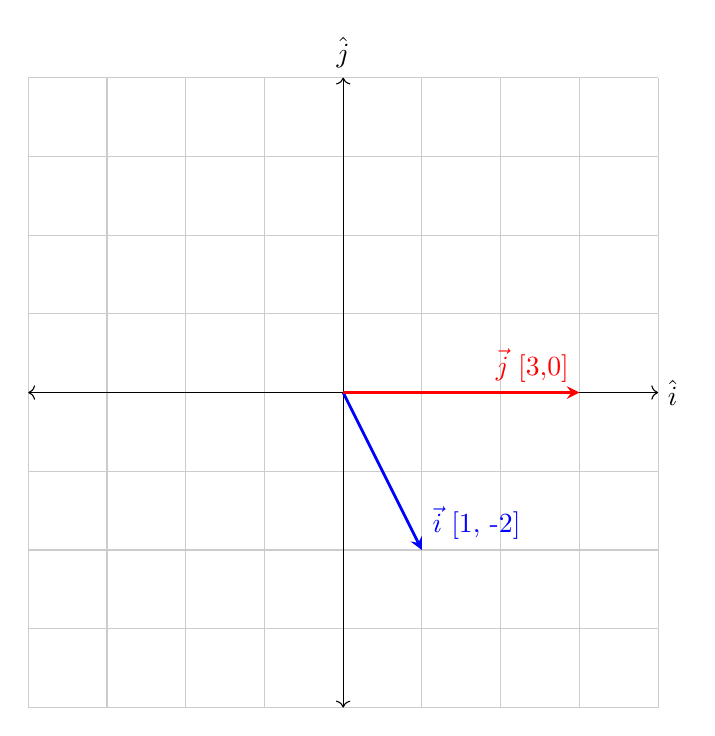
\begin{tikzpicture}
	\draw[thin,gray!40] (-4,-4) grid (4,4);
	\draw[<->] (-4,0)--(4,0) node[right]{$\hat{i}$};
	\draw[<->] (0,-4)--(0,4) node[above]{$\hat{j}$};
	\draw[line width=1pt,blue,-stealth](0,0)--(1,-2) node[anchor=south west]{$\vec{i}$	[1, -2]};
	\draw[line width=1pt,red,-stealth](0,0)--(3,0) node[anchor=south east]{$\vec{j}$	[3,0]};
\end{tikzpicture}
The new basis vectors are blue $\vec{i}$ and red $\vec{j}$.
\\
\\
Now in this new transformed space, every vector has to be represented as a linear combination of these two new basis vectors.
\\
\\
The vector $\vec{v} =$ -1$\hat{i} + 2 \hat{j}$ after transformation lands at the point $\tcomat{5}{2}$ in the new vector space.
\\
\\
Even after the transformation, the linear combination doesn't change. So, $\hat{i}$ and $\hat{j}$ are replaced by $\tcomat{1$\hat{i}$}{-2$\hat{j}$}$ and 	$\tcomat{3$\hat{i}$}{0$\hat{j}$}$ respectively.
\\
\\
So the new transformed $\vec{v}$ becomes,
\begin{equation}
	\vec{v}_{new}  = -1\hat{i}_{new} + 2 \hat{j}_{new}
\end{equation}
\begin{equation}
		\vec{v}_{new}  = -1\tcomat{1$\hat{i}$}{-2$\hat{j}$} + 2\tcomat{3$\hat{i}$}{0$\hat{j}$}
\end{equation}
\begin{equation}
			\vec{v}_{new}  =\tcomat{-1$\hat{i}$}{2$\hat{j}$} + \tcomat{6$\hat{i}$}{0$\hat{j}$}
\end{equation}

\begin{equation}
	\vec{v}_{new}  = \tcomat{5$\hat{i}$}{2$\hat{j}$}
\end{equation}
For any vector $x\hat{i}+y\hat{j}$, after applying the transformation $\begin{bmatrix}
	1 & 3\\
	$-2$ & 0
\end{bmatrix}$ becomes,
\begin{equation}
	 \begin{bmatrix}
		x \hat{i}\\
		y \hat{j}
		\end{bmatrix}  \overset{lr. \; transform}{ \implies }  x \begin{bmatrix}
		1 \hat{i}\\
		$-2$ \hat{j}
	\end{bmatrix} + y \begin{bmatrix}
	3 \hat{i}\\
	0 \hat{j}
\end{bmatrix} = \begin{bmatrix}
1x+3y \hat{i}\\
-2x+0y \hat{j}
\end{bmatrix} 
\end{equation}
Removing $\hat{i}$, $\hat{j}$ for legibility,
\begin{equation}
	\begin{bmatrix}
		x \\
		y 
	\end{bmatrix}  \overset{lr. \; transform}{ \implies }  x \begin{bmatrix}
		1 \\
		$-2$ 
	\end{bmatrix} + y \begin{bmatrix}
		3 \\
		0
	\end{bmatrix} = \begin{bmatrix}
		1x+3y\\
		-2x+0y
	\end{bmatrix} 
\end{equation}

This is the basis for Matrix multiplication.
\begin{itemize}
	\item $\begin{bmatrix}
		1 \\
		$-2$ 
	\end{bmatrix}$ is where $\hat{i}$ lands and $\begin{bmatrix}
	3 \\
	0 
\end{bmatrix}$ is where $\hat{j}$ (basis vectors) lands after the transformation.
\item So the 2X2 matrix $\begin{bmatrix}
	1 & 3\\
	$-2$ & 0
\end{bmatrix}$ itself can represent the transformation.
\item This explains the \emph{rules} for multiplication and why matrix multiplication is not commutative.
\item This also explains why the matrix $\begin{bmatrix}
	1 & 0\\
	0 & 1
\end{bmatrix}$ is an identity matrix. Since, this \emph{transform} actually does nothing, $\hat{i}$ and $\hat{j}$ remain unchanged.
\end{itemize}

For any transformation $\begin{bmatrix}
	a & b\\
	c & d
\end{bmatrix}$,
\begin{equation} \label{eq:transform1}\underbracket{
	 \begin{bmatrix}
		a & b\\
		c & d
	\end{bmatrix}}_{\mathclap{Transformation}} \overbracket{\begin{bmatrix}
	x\\
	y
\end{bmatrix}}^{old \; vector}=x  \overbracket{\begin{bmatrix}
a\\
c 
\end{bmatrix}}^{\mathclap{where \; \hat{i} \;  lands}} + y \underbracket{\begin{bmatrix}
b\\
d
\end{bmatrix}}_{\mathclap{where \; \hat{j} \; lands}} = \overbracket{\begin{bmatrix}
ax+by\\
cx+by
\end{bmatrix}}^{\mathclap{Transformed \; matrix}}
\end{equation}
\begin{itemize}
	\item $\begin{bmatrix}
		a\\
		c
	\end{bmatrix}$ and $\begin{bmatrix}
	b\\
	d
\end{bmatrix}$ are the new basis vectors; where old $\hat{i}$ and $\hat{j}$ land. These are the new transformed basis vectors.

\item Now these new basis vectors have to be used to represent all the vectors in it's span. In other words the linear combination of these two basis vectors.

\item From equation \ref{eq:transform1} it can be observed that the scalars $x$  and $y$ scale the corresponding new basis vectors.

	\item For no transformation (or) Identity transform / Multiplication,
	\begin{equation}
		\tctmat{1}{0}{0}{1} \tcomat{x}{y} = \tcomat{x}{y}
	\end{equation}
	Which makes sense !!
\end{itemize}

\hformbar
\formdesc{Counterclock Transform:}\\

$\tctmat{0}{-1}{1}{0}$ $\tcomat{x}{y}$


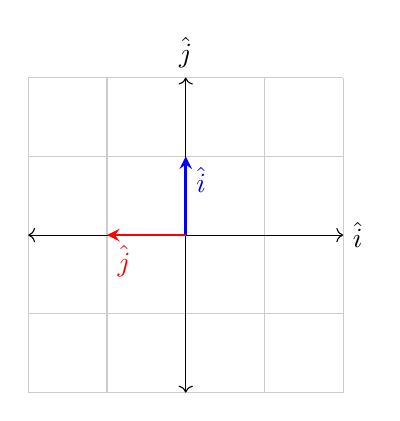
\begin{tikzpicture}
	\draw[thin,gray!40] (-2,-2) grid (2,2);
	\draw[<->] (-2,0)--(2,0) node[right]{$\hat{i}$};
	\draw[<->] (0,-2)--(0,2) node[above]{$\hat{j}$};
	\draw[line width=1pt,blue,-stealth](0,0)--(0,1.0) node[anchor=north west]{$\hat{i}$};
	\draw[line width=1pt,red,-stealth](0,0)--(-1,0) node[anchor=north west]{$\hat{j}$};
\end{tikzpicture}

\hformbar
\formdesc{Shear Transform:}\\

$\tctmat{1}{1}{0}{1}$ $\tcomat{x}{y}$


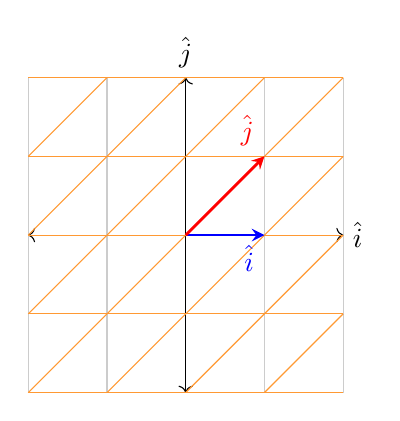
\begin{tikzpicture}
	\draw[thin,gray!40] (-2,-2) grid (2,2);
	\draw[<->] (-2,0)--(2,0) node[right]{$\hat{i}$};
	\draw[<->] (0,-2)--(0,2) node[above]{$\hat{j}$};
	
	%new grid
	%horizontal
	\foreach \y in {-2,...,2}
	{\draw[orange!80] (-2,\y)--(2,\y);}
	%vertical
	\draw[orange!80] (-2,1)--(-1,2);
	\draw[orange!80] (-2,0)--(0,2);
	\draw[orange!80] (-2,-1)--(1,2);
	\draw[orange!80] (-2,-2)--(2,2);
	\draw[orange!80] (-1,-2)--(2,1);
	\draw[orange!80] (0,-2)--(2,0);
	\draw[orange!80] (1,-2)--(2,-1);
	
	\draw[line width=1pt,blue,-stealth](0,0)--(1,0) node[anchor=north east]{$\hat{i}$};
	\draw[line width=1pt,red,-stealth](0,0)--(1,1) node[anchor=south east]{$\hat{j}$};
\end{tikzpicture}

\hformbar
\formdesc{Few notable points:}\\

\begin{itemize}
	\newcommand\ii{$\tcomat{2}{1}$}
	\newcommand\jj{$\tcomat{-2}{-1}$}
	\item In transformations, order matters. $M_1M_2 \neq M_2M_1$ because $f(g(x)) \neq g(f(x))$
	\item The associative property $(AB)C = A(BC)$ holds true because the order is $C$, $B$ then $A$ regardless.
	\item For a $\tctmat{2}{-2}{1}{-1}$ transformation all 2d space is squished into a line.
	
	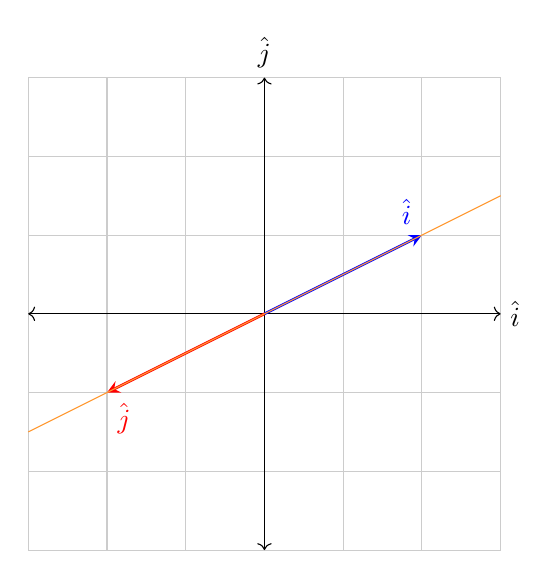
\begin{tikzpicture}
	\draw[thin,gray!40] (-3,-3) grid (3,3);
	\draw[<->] (-3,0)--(3,0) node[right]{$\hat{i}$};
	\draw[<->] (0,-3)--(0,3) node[above]{$\hat{j}$};
	\draw[line width=1pt,blue,-stealth](0,0)--(2,1) node[anchor=south east]{$\hat{i}$	\ii};
	\draw[line width=1pt,red,-stealth](0,0)--(-2,-1) node[anchor=north west]{$\hat{j}$	\jj};
	\draw[orange!80] (-3,-1.5)--(3,1.5);
	\end{tikzpicture}

These two vectors \ii and \jj are linearly dependent vectors.
\item Two transforms for ex. shear and rotation can be composed into a single transform. This composition transform is nothing but a multiplication of shear and rotation matrix.
	\begin{equation}
	\underbracket{\tctmat{1}{1}{0}{1}}_{\mathclap{Shear}}
	\overbracket{ \tctmat{0}{-1}{1}{0}}^{\mathclap{Rotation}} \tcomat{x}{y} = 
	\underbracket{\tctmat{1}{-1}{1}{0}}_{\mathclap{Compostion}} \tcomat{x}{y}
	\end{equation}
\item Product or composition of two matrices/ transforms,
\begin{equation}
	\tctmat{a}{b}{c}{d} \tctmat{e}{f}{g}{h} = \tctmat{ae$+$bg}{af$+$bh}{ce$+$dg}{cf$+$dh}
\end{equation}

\end{itemize}

\hformbar
\formdesc{Determinant:}
\begin{itemize}
	\item Transformation $\tctmat{3}{0}{0}{2}$ scales $\hat{i}$ by factor 3 $\hat{j}$ by a factor 2.
\end{itemize}
\begin{figure}[ht!]
		\centering
		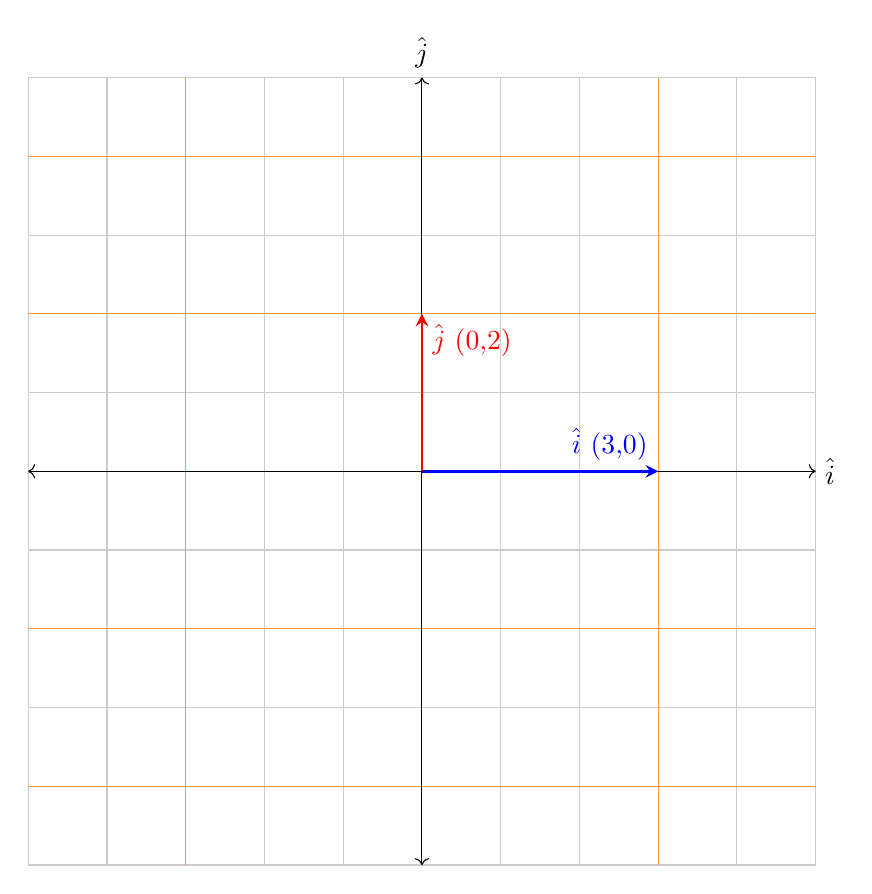
\begin{tikzpicture}
		\draw[thin,gray!40] (-5,-5) grid (5,5);
		% new grid
		\foreach \x in {-3,0,3}
		{\draw[orange!80] (\x,-5)--(\x,5);}
		\foreach \y in {-4,-2,...,4}
		{\draw[orange!80] (-5,\y)--(5,\y);}
		% axis
		\draw[<->] (-5,0)--(5,0) node[right]{$\hat{i}$};
		\draw[<->] (0,-5)--(0,5) node[above]{$\hat{j}$};
		% vector
		\draw[line width=1pt,blue,-stealth](0,0)--(3,0) node[anchor=south east]{$\hat{i}$ (3,0)};
		\draw[line width=1pt,red,-stealth](0,0)--(0,2) node[anchor=north west]{$\hat{j}$ (0,2)};
	\end{tikzpicture}
\end{figure}


\begin{itemize}
	\item We observe that the unit square in transformed space is scaled from 1 sq. unit to 6 sq. units. So the determinant of the transform/matrix $\tctmat{3}{0}{0}{2}$ is 6. In case of 3d, volume is scaled.
	\item For a matrix/transform $\tctmat{a}{b}{c}{d}$, the determinat is $ad-bc$.
	\item The determinant can be $-ve$ if the axis cross each other during the transformation. It has the effect of \emph{flipping} or \emph{inverting} the space.
	
	
	% Credit https://i.stack.imgur.com/0hxY1.png https://stackoverflow.com/a/34068511/4915164
	\begin{figure}[ht!]
		\graphicspath{ {images/math/} }
		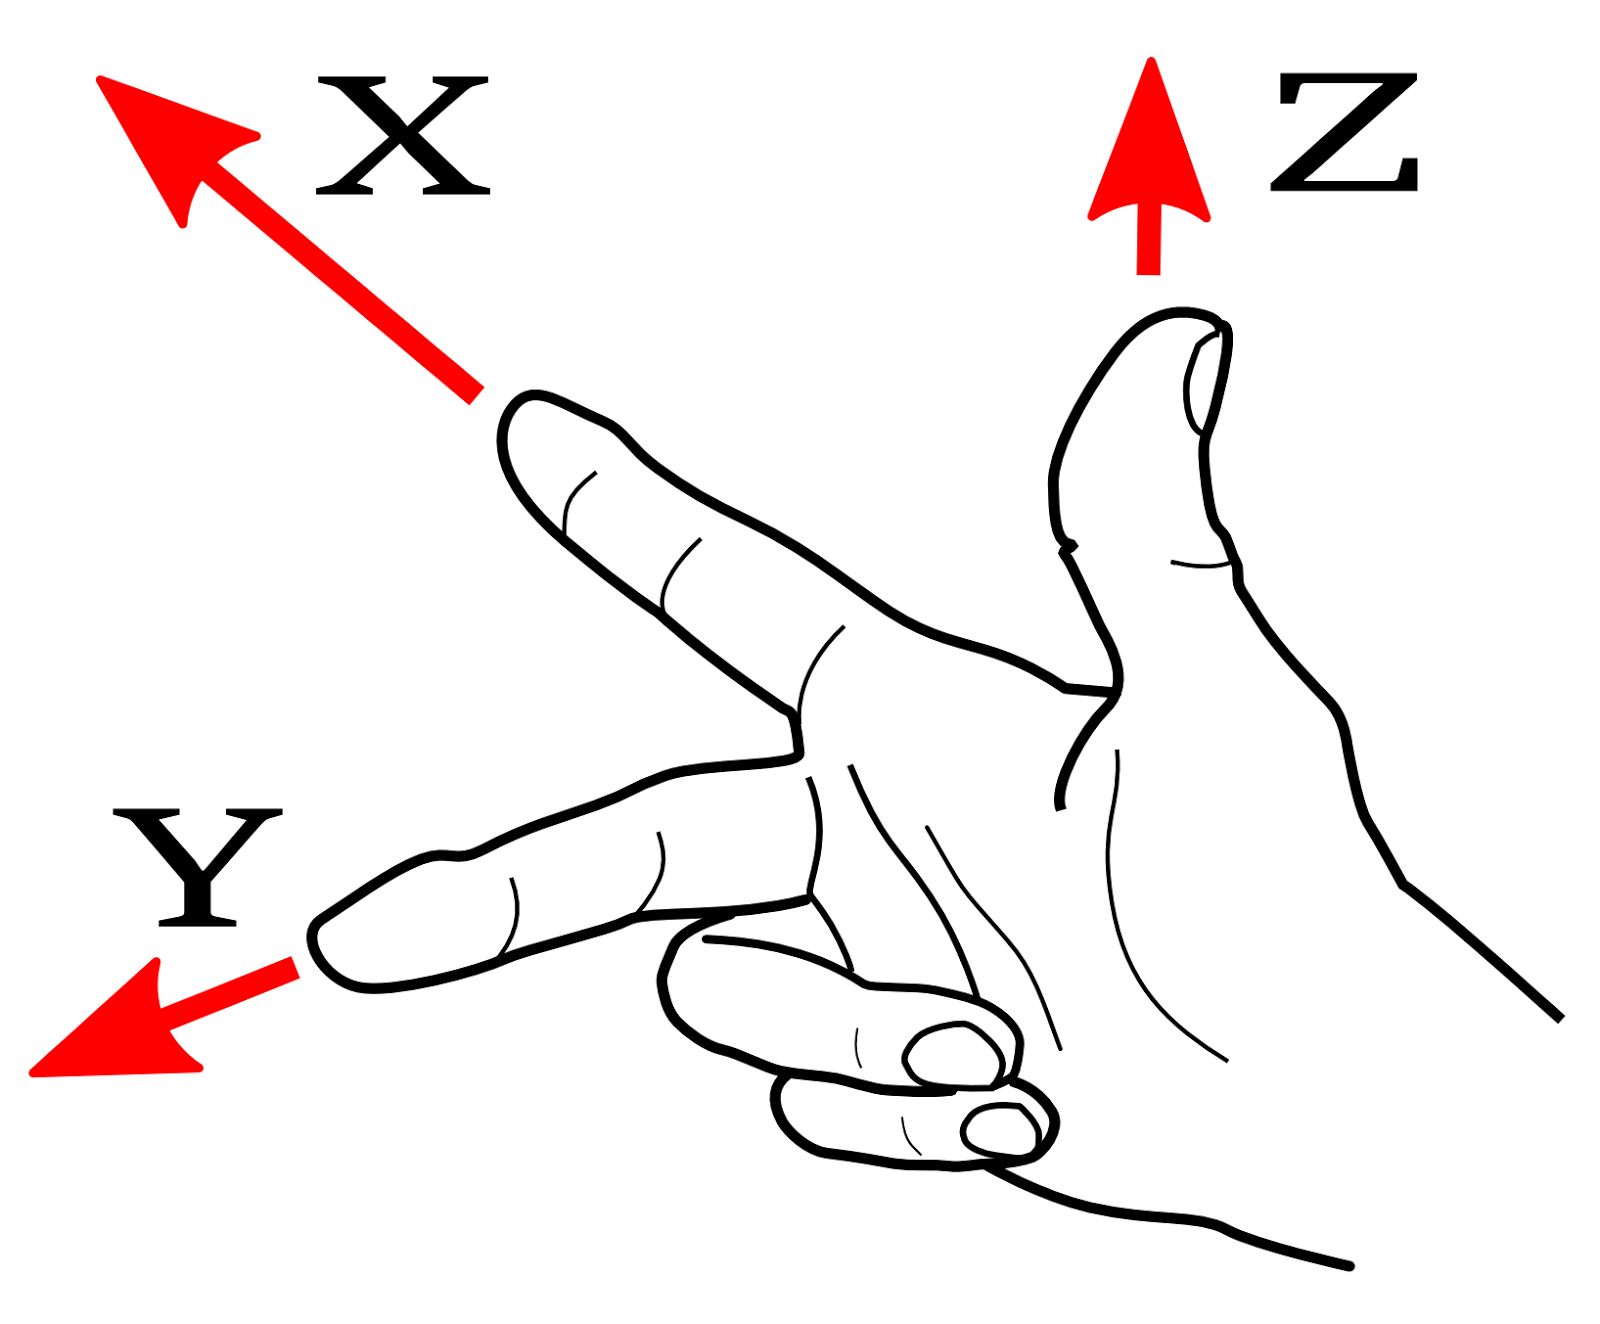
\includegraphics[width=\linewidth]{right-hand-rule.png}
	\end{figure}
	\item This can be checked using right hand rule to check if the axis still lie in the same orientation after transformation. If not, the determinant is $-ve$.
	\item For 3d space, determinant is measured by unit volume instead of area.
	\item Determinant can be zero if the space is squished. For ex. if transformed to a line or point in 2d or to a plane, line or a point in 3d. This has the effect of reduction in number of dimensions.
\end{itemize}

\begin{equation}
	det(M_1M_2) = det(M_1)  det(M_2)
\end{equation}


\hformbar
\formdesc{System of equations:}
\\


$A.\vec{X} = \vec{V}$\\

$3x+1y+4z = 1$

$3x+9y+2z = 6$

$3x+3y+3z = 8$

\begin{itemize}
	\item Solving these system of equations imply, finding the vector $\thcomat{x}{y}{z}$ that if applied the transformation $\thcthmat{3}{1}{4}{3}{9}{2}{3}{3}{3}$, would land on the vector $\thcomat{1}{6}{8}$.
	
	\item This can only be solved if $A^{-1}$ exists. Since space cannot be unpacked since there is/are lost dimension(s) if $det(A) = 0$. So $det(A) \neq 0$ has to be true for the system of equations to be solved using,
	
	\begin{equation}
		\vec{X} = A^{-1}\vec{V}
	\end{equation}
\end{itemize}

\hformbar
\formdesc{Rank:}
\begin{itemize}
	\item Rank is the number of dimensions of the transformed space.
	\item The Rank of a matrix ; output space.
	
	Rank : 1 $\implies$ output transformation : Line
	
	Rank : 2 $\implies$ output transformation : Plane
	
	Rank : 0 $\implies$ output transformation : Point
\end{itemize}


\hformbar
\formdesc{Column space:}

\begin{itemize}
	\item Set of all possible linear combinations or span of column vectors of $A$. Or,
	\item Set of all possible $A \vec{V}$
\end{itemize}

\hformbar
\formdesc{Null space:}
\begin{itemize}
	\item Set of vectors that get squished into origin after transformation.
\end{itemize}

\hformbar
\formdesc{Dot Product:}
\begin{itemize}
	\item $\vec{a}$ and $\vec{b}$ are two vectors and angle between them is $\theta$.
	
	\begin{equation}
		\vec{a} = [a_1 ,a_2 ,... a_n]
	\end{equation}
	\begin{equation}
		\vec{b} = [b_1, b_2,... b_n]
	\end{equation}
	\begin{equation}
		\vec{a}.\vec{b} = (a_1)*(b_1) + (a_2)*(b_2) + ... + (a_n)*(b_n)
	\end{equation}
	
	\item Geometric representation:
	\begin{equation}
		\vec{a}.\vec{b} = ||{a}||* ||{b}||* cos \theta
	\end{equation}
	
	\begin{tikzpicture}
		\coordinate (o) at (0,0);
		\draw[.->] (0,0)--(5,0)  coordinate (a) node[right]{$\vec{a}$};
		\draw[.->] (0,0)--(3,4)  coordinate (b)  node[above]{$\vec{b}$};
		\pic [draw, ->, "$\theta$", angle eccentricity=1.5] {angle =a--o--b};
	\end{tikzpicture}
	
	dot product of two vectors = (length of any vector) x 
	(length of projection made on the vector)
	
\end{itemize}


\newcommand{\dotbase}{
	\coordinate (o) at (0,0);
	\draw[thin,gray!40] (-2,-2) grid (6,4);
	\draw[<->] (-2,0)--(6,0) node[right]{$\hat{i}$};
	\draw[<->] (0,-2)--(0,4) node[above]{$\hat{j}$};
	\draw[line width=1pt,blue,-stealth](0,0)--(2,2) coordinate (a) node[anchor=south east, pos=0.8]{$\vec{a}$	[2,2]};
	\draw[line width=1pt,red,-stealth](0,0)--(4,-1) coordinate (b) node[anchor=south west]{$\vec{b}$	[4,-1]};
	\pic [draw, ->, "$\theta$", angle eccentricity=1.5] {angle =b--o--a};
}

\begin{tikzpicture}
	\dotbase
\end{tikzpicture}
\\
\\

Projecting $\vec{a}$ on $\vec{b}$:

\begin{tikzpicture}
	\dotbase
	\draw[dashed] (2,2)--(1.411764,-0.352941176) coordinate(p);
	\draw [decorate,decoration={brace,amplitude=10pt,mirror,raise=2pt},yshift=0pt]
	(0,0) -- (1.411764,-0.352941176) node [black,midway,xshift=0pt, yshift=-25pt,rotate=-13] {\footnotesize
		length of projection};
        \tkzMarkRightAngle[draw=black,size=.2](o,p,a);
        
\end{tikzpicture}

\begin{itemize}
	\item Length of projection = $||a||cos\theta$
	\item Dot product = $||b||.||a|| cos\theta $
	\item The length of projection does not depend on the length of $\vec{b}$. It only depends on length of $\vec{a}$ and $\theta$.
	\item Projecting $\vec{b}$ on $\vec{a}$ will result in the same dot product result. The order does not matter.
	\item If projection does not lie betweeon origin and the end point of the other vector, you can extend the other vector since length of projection is not affected by it.
	\item Dot product is -ve if projection is on -ve side.
\end{itemize}

\hformbar
\formdesc{Cross Product:}

\begin{itemize}
	\item Directed area product.
	%https://en.wikipedia.org/wiki/Cross_product#/media/File:Cross_product_parallelogram.svg
		\begin{figure}[ht!]
		\graphicspath{ {images/math/} }
		\includesvg[width=\linewidth]{cross_product_parallelogram}
	\end{figure}

	% https://en.wikipedia.org/wiki/Cross_product#/media/File:Right_hand_rule_cross_product.svg
	\begin{figure}[ht!]
		\graphicspath{ {images/math/} }
		\includesvg[width=\linewidth]{right_hand_rule_cross_product}
	\end{figure}

	\item $\vec{a}\times \vec{b} = -\vec{b} \times \vec{a}$
	\item Length of $\vec{a}\times \vec{b}$ = $det (\tctmat{$a_1$}{$b_1$}{$a_2$}{$b_2$})$
	\item The cross product vector is normal to the area.
	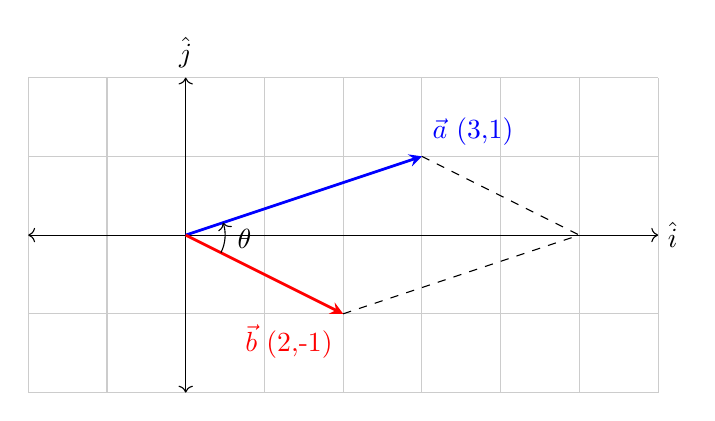
\begin{tikzpicture}
		\coordinate (o) at (0,0);
		\draw[thin,gray!40] (-2,-2) grid (6,2);
		\draw[<->] (-2,0)--(6,0) node[right]{$\hat{i}$};
		\draw[<->] (0,-2)--(0,2) node[above]{$\hat{j}$};
		\draw[line width=1pt,blue,-stealth](0,0)--(3,1) coordinate (a) node[anchor=south west]{$\vec{a}$	(3,1)};
		\draw[line width=1pt,red,-stealth](0,0)--(2,-1) coordinate(b) node[anchor=north east]{$\vec{b}$	(2,-1)};
		\draw[dashed] (2,-1)--(5,0);
		\draw[dashed] (3,1)--(5,0);
		\pic [draw, ->, "$\theta$", angle eccentricity=1.5] {angle =b--o--a};
	\end{tikzpicture}
	\item The area of this parallelogram is $det (\tctmat{3}{2}{1}{-1})$
	\item The direction of the cross product is normal to the area, i.e, in the direction of $\hat{k}$
	\item The magnitude of this vector is the area of this parallelogram i.e, determinant.
	\begin{equation}
		\vec{a} \times \vec{b} = ||a|| . ||b|| sin\theta
	\end{equation}
\end{itemize}


\hformbar
\formdesc{Eigen:}
\begin{itemize}
	\item For a few transformations, vectors only scale. i.e, only stretch or compress.
	\item Such vectors are called eigen vectors of the transformation.
	\item Such vectors are transformed into it's own span.
	\item The scaled value of such vectors (scalar) is the eigen value. It can be +ve or -ve.
	\begin{equation}
		A\vec{V} = \lambda \vec{V}
	\end{equation}
where:

	$A$ is the transformation,
	
	$\vec{V}$ is the eigen vector and,
	
	$\lambda$ is the eigen value.
\end{itemize}


\hformbar
\formdesc{Vector from origin:}\\
\begin{itemize}
	\item As discussed previously, any vector can be moved to origin for reference, without changing it's direction it is pointing to and it's length.
	\item To make a vector starting from $\thcomat{$a_1$}{$a_2$}{$a_3$}$ and ending at $\thcomat{$b_1$}{$b_2$}{$b_3$}$ as a reference vector, we can apply triangular law of addition to get a vector which starts from origin and is equivalent with the vector starting and ending at the above two points.
	\item We need to remember that the above vectors themselves start at origin. So, we can get the vector by doing $\thcomat{$a_1$}{$a_2$}{$a_3$}$ $-$ $\thcomat{$b_1$}{$b_2$}{$b_3$}$
\end{itemize}

\hformbar
\formdesc{Matrices:}\\

Diagonal Matrix:
\begin{itemize}
	\item A matrix with all 0's except diagonal elements.
\end{itemize}

\hformbar

Identity Matrix:
\begin{itemize}
	\item A Matrix with all diagonal elements as 1.
	
	$I = \thcthmat{1}{0}{0}{0}{1}{0}{0}{0}{1}$
\end{itemize}

\hformbar

Scalar Matrix:
\begin{itemize}
	\item A Matrix with only equal diagonal elements.
	\item A scalar matrix can be represented by a single scalar.
	
	$K.I = \thcthmat{4}{0}{0}{0}{4}{0}{0}{0}{4}$
\end{itemize}
\hformbar

Upper Triangular Matrix:
\begin{itemize}
\item A Matrix with all elements below diagonal are 0

$\thcthmat{3}{5}{2}{0}{2}{7}{0}{0}{1}$
\end{itemize}

\hformbar

Lower Triangular Matrix:
\begin{itemize}
	\item A Matrix with all elements above diagonal are 0
	
	$\thcthmat{3}{0}{0}{7}{2}{0}{5}{3}{1}$
\end{itemize}

\hformbar

Symmetric Matrix:
\begin{itemize}
	\item A square matrix which is equal to its transpose.
	\item $A=A^T$
	\item $a_{ij} = a_{ji}$ for every i and j.
	
%https://en.wikipedia.org/wiki/Symmetric_matrix#/media/File:Matrix_symmetry_qtl1.svg
	\begin{center}
		\graphicspath{ {images/math} }
		\includesvg[width=\linewidth]{matrix_symmetry.svg}
	\end{center}

\end{itemize}


\hformbar

Skew Symmetric Matrix:
\begin{itemize}
	\item A square matrix which is equal to negative of its transpose.
	\item $A=-A^T$
	\item $a_{ij} = -a_{ji}$ for every i and j.
\end{itemize}


\hformbar

Orthogonal Matrix:
\begin{itemize}
	\item A square matrix whose column vectors and row vectors are orthonormal.
	\item $AA^T=A^TA=I$ or,
	\item $A^T=A^{-1}$
	\item $a_{ij} = -a_{ji}$ for every i and j.
\end{itemize}


\hformbar
\formdesc{Lines, Planes and Hyperplanes:}
\begin{itemize}
	\item  \textbf{Line} - A line has 2 degrees of freedom. You need a point and a slope or two points to uniquely identify a line.
	\item Equation of a line
	\begin{enumerate}
		\item $y=mx+c$ ; slope = m ; y - intercept = c ; passes through $(0,c)$
		\item $ax+by+c=0$ is a simple linear form with 2 unknowns
		\item $y-y_1=m(x-x_1)+c$ ; slope = m ; passes through $x_1$ and $y_1$
	\end{enumerate}
	\item Slope is the $tan$ of angle x axis makes with the line in anti-clock wise direction.
	\item Any 2 points on a line can uniquely identify the line.
	\item An object on a line can move in 1 dimension.
\end{itemize}

\hformbar

\begin{itemize}
	\item \textbf{Plane} - A plane is a flat 2d surface.
	\item A $xy$ plane is an example of a plane.
	\item To represent a plane you need 3 non collinear points or a point and a normal.
	\item A normal is a vector that is perperndicular to all vectors on the surface.
	\begin{enumerate}
		\item So, by definition a plane is set all $(x,y,z)$ points that satisfy,
					\begin{equation}
						dot(\thcomat{$x$}{$y$}{$z$} - \thcomat{$x_0$}{$y_0$}{$z_0$}, \vec{n}) = 0
					\end{equation}
				Where:
				
					$\vec{n}=\thcomat{$n_1$}{$n_2$}{$n_3$}$ is the normal to the plane and  starts at point $\thcomat{$x_0$}{$y_0$}{$z_0$}$ which is located on the plane.
	\end{enumerate}
	\item The equation subsequently solves to,
		\begin{equation}
			n_1(x-x_0) + n_2(y-y_0) + n_3(z-z_0) = 0
		\end{equation}
		\begin{figure}[ht!]
	\graphicspath{ {images/math/} }
	\includesvg[width=\linewidth]{plane}
	\end{figure}
\end{itemize}

\hformbar

\begin{itemize}
	\item \textbf{Hyperplane} - Is an extension to Line and a plane in higher dimensions.
\end{itemize}

\hformbar

\begin{itemize}
	\item A \textbf{Linear regression} model can successfully represent a line, plane or a hyperplane.
\end{itemize}

\hformbar
\formdesc{Miscellaneous:}
\begin{itemize}
	\item Distance between two points $(x_1,y_1)$ and $(x_2,y_2)$ is $$\sqrt{(x_2-x_1)^2 + (y_2-y_1)^2}$$
	\item Length of a vector $a\hat{i}+b\hat{j}+c\hat{k}$ is $$\sqrt{a^2+b^2+c^2}$$ also known as L2 Norm. {\scriptsize (Check knn notes for info on norms.)}
	\item Distance from a plane $ax+by+cz=0$ to a point $(x_1,y_1)$ is $$\frac{|ax_1+by_1+cz_1|}{\sqrt{a^2+b^2+c^2}}$$
\end{itemize}

\hformbar
\formdesc{Credits:}
\begin{itemize}
	\item Most of this notes is taken from 3Blue1Brown's Essence of Linear Algebra playlist. Some images are taken from wikipedia.
\end{itemize}

\newpage
\section{Probability}


\hformbar
\formdesc{Population and Sample:} 
\begin{itemize}
	\item (Statistical) population is a set of all the items or events which is of interest for a question or experiment.
	\item (Statistical) sample is a subset of population. The aim of sampling is that our sample represents the population.\\ The advantage is that it is faster and cheaper to collect data than for the entire population.
	
	%https://en.wikipedia.org/wiki/Sampling_(statistics)#/media/File:Simple_random_sampling.PNG
	\begin{figure}[ht!]
		\caption{A random sampling process}
		\graphicspath{ {images/math/} }
		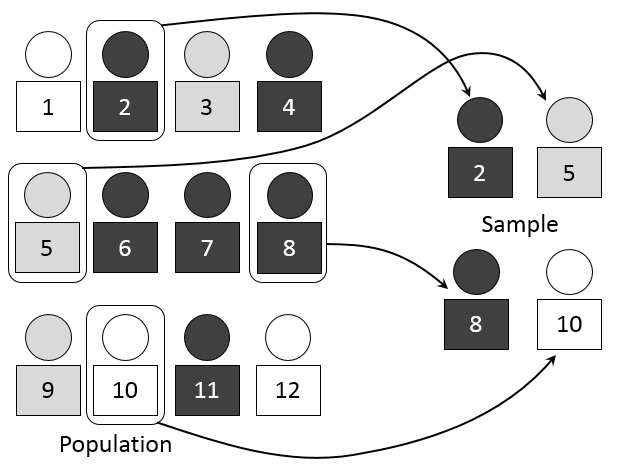
\includegraphics[width=\linewidth]{simple_random_sampling}
	\end{figure}
	
	\begin{figure}[ht!]
		\centering
		\caption{A sample is a subset of population}
		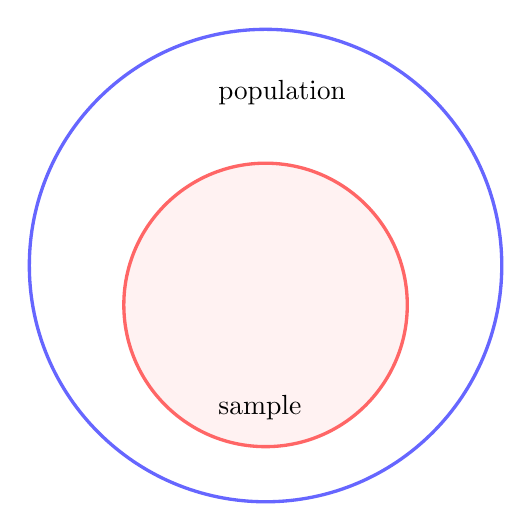
\begin{tikzpicture}
			\filldraw[color=blue!60, fill=white!2, very thick](0,0) circle (3.0);
			\filldraw[color=red!60, fill=red!5, very thick](0,-0.5) circle (1.8);
			\node[text width=1.2cm] at (0,-1.8) {sample};
			\node[text width=1.2cm] at (0,2.2) {population};
		\end{tikzpicture}
	\end{figure}
\end{itemize}

\newpage
\hformbar
\formdesc{Random variable:} ($X$)

\begin{itemize}
	\item A Random variable is a measurable function defined on probability space that maps from the sample space to real numbers.
	\item It is called a \textbf{Discrete Random variable} if the range of the function is countable.
	\item It is called a \textbf{Continous Random variable} if the range of the function is uncountably infinite or an interval.
	\item Both these types of  Random variable has a distribution.
		\begin{itemize}
			\item If $X$ is a \textbf{Discrete Random variable}, it's distribution is a discrete probability distribution i.e. can be described by a probability mass function (pmf) that assigns a probability to each value in the range of  $X$.
			\item If $X$ is a \textbf{Continous Random variable}, and \emph{absolutely continuous}, its distribution can be described by a probability density function (pdf).\\ Pdf assigns probailities to an interval and since the range is absolutely continuous, each individual point must have a probability of 0.
		\end{itemize}
	\item Not all continuous random variables are absolutely continuous.\\ A mixture distribution is one such counterexample; such random variables cannot be described by a probability density or a probability mass function. 
	\item But all Random variable can be described by a Cumulative distribution function (cdf).
	\item Ex. for a discrete rv is dice rolls and for continuous rv is height or incomes of people.
\end{itemize}


\hformbar
\formdesc{Probability Distribution:}

\begin{itemize}
	\item A Probability Distribution is  the mathematical function that gives probabilities of occurences of different possible outcomes for an experiment.
	\item It is a mathematical description of a random phenomenon in terms of its  sample space and the probabilities of events (subsets of the sample space).
\end{itemize}

\newpage
\hformbar
\formdesc{Probability Density Function (pdf):}
\begin{itemize}
	\item Pdf is a function used to specify the random variable falling within a particular range of values, as opposed to taking any particular value(which is 0, since there are infinite number of values).
	\item Probablity is the integral or area under the curve over an interval.
	\item It's value at any given point can be interpreted as providing the relative likelyhood that the value of the random variable would equal that sample.
	\item In other words, while the absolute likelihood for a continuous random variable to take on any particular value is 0 (since there is an infinite set of possible values to begin with), the value of the PDF at two different samples can be used to infer, in any particular draw of the random variable, how much more likely it is that the random variable would equal one sample compared to the other sample. 
\end{itemize}
Properties of pdf:
\begin{itemize}
	\item Area under the curve or AUC(pdf) = 1
	\item Value at any point of pdf curve has to be $\geq0$
	\item x-axis : Random variable $X$ \\ y-axis : Relative likelyhood/ probability density.
	\item For a continuous rv, it's pdf has to also be continuous.
	\item A pdf doesn't have to be differentiable. For ex. Laplace distribution is not differentiable. $$\frac{1}{2}e^{-|x|}$$
	\item But a CDF has to be differentiable.
	\item A point on pdf provides relative likelyhood. Whereas, area under an interval gives probability.
	\item Few random variables may not have pdf. They are called Singular distributions.
\end{itemize}

\newpage
\hformbar
\formdesc{Gaussian/ Normal Distribution:} ($N$)
\begin{equation}
	P(X=x) = \frac{1}{\sqrt{2\pi}\sigma} \exp{\frac{-(x-\mu)^2}{2\sigma^2}}
\end{equation}
where:

	$\mu$ - Mean or expectation
	
	$\sigma$ - Standard deviation
	
	$\sigma^2$ - Variance
	
\begin{itemize}
	\item The significance of Normal distribution comes from various factors like,
		\begin{itemize}
			\item Central limit theorem
			\item Many natural properties follow a roughly Normal distribution
			\item For a fixed mean and std. deviation, Normal disitribution has maximum entropy.
		\end{itemize}
	\item Though Normal distribution is commonly referred to as a bell curve, there are also other distributions in the bell curve family.
\end{itemize}


	%https://en.wikipedia.org/wiki/Normal_distribution#/media/File:Normal_Distribution_PDF.svg
\begin{figure}[ht!]
	\centering
	\caption{pdf of a normal distribution}
	\graphicspath{ {images/math/} }
	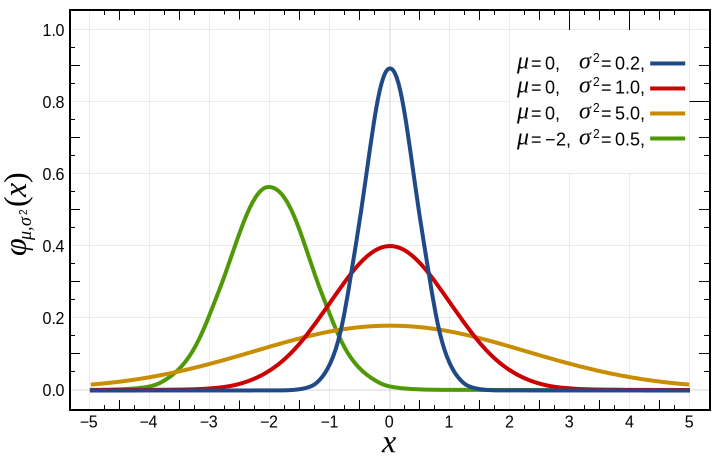
\includegraphics[width=\linewidth]{normal_distribution_pdf}
\end{figure}

%https://en.wikipedia.org/wiki/Normal_distribution#/media/File:Normal_Distribution_CDF.svg
\begin{figure}[ht!]
	\centering
	\caption{cdf of a normal distribution}
	\label{fig:cdf-normal}
	\graphicspath{ {images/math/} }
	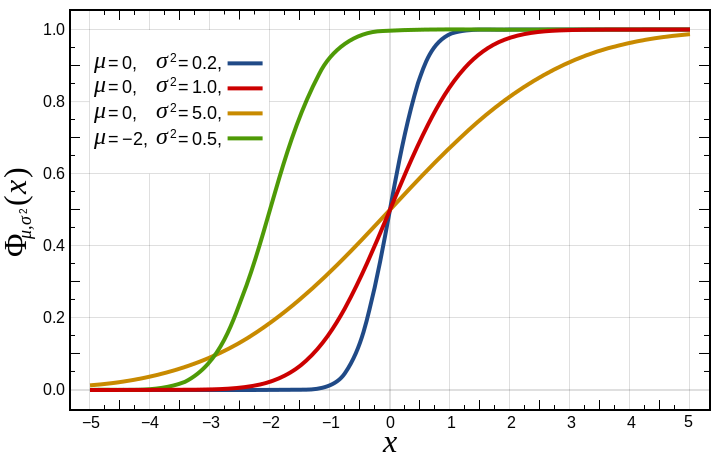
\includegraphics[width=\linewidth]{normal_distribution_cdf}
\end{figure}

\newpage
68-95-99.7 Rule:

\begin{itemize}
	\item It is an empirical rule that a percentage of values lie within a band around the mean for a normal distribution.
		
	%https://en.wikipedia.org/wiki/Statistics#/media/File:Standard_Normal_Distribution.png
	\begin{figure}[ht!]
		\caption{pdf of a standard normal distribution}
		\graphicspath{ {images/math/} }
		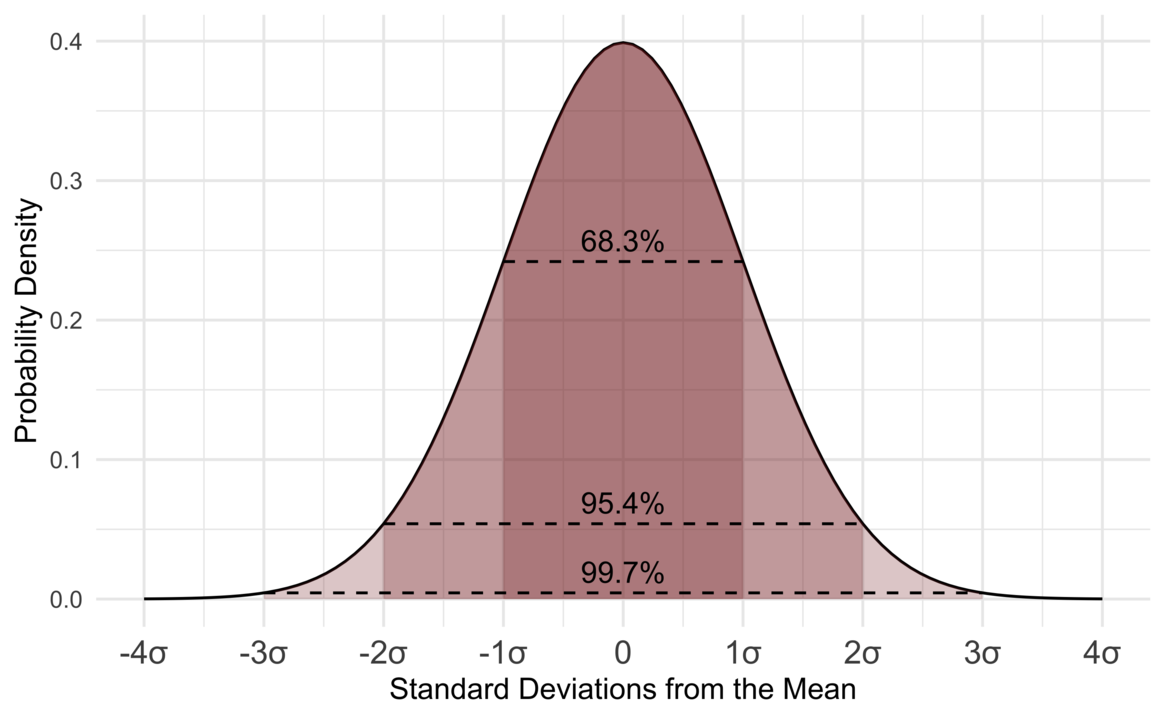
\includegraphics[width=\linewidth]{standard_normal_distribution}
	\end{figure}
	\item The percentage of values are,
		\begin{itemize}
			\item 68\% of values lie within $\mu-1\sigma$ and $\mu+1\sigma$
			\item 95\% of values lie within $\mu-2\sigma$ and $\mu+2\sigma$
			\item 99.7\% of values lie within $\mu-3\sigma$ and $\mu+3\sigma$
		\end{itemize}
	
	\item Is valid for any value of $\mu$ and $\sigma$
	%https://en.wikipedia.org/wiki/Statistics#/media/File:Standard_Normal_Distribution.png
	\begin{figure}[ht!]
		\caption{pdf of a normal distribution with mean $\mu$ and std-dev. $\sigma$}
		\graphicspath{ {images/math/} }
		\includesvg[width=\linewidth]{empirical_rule_histogram}
	\end{figure}
\end{itemize}

\newpage

\hformbar
\formdesc{Cumulative distribution function:} (CDF)

\begin{itemize}
	\item The probability that rv $X$ will take a value less than $x$. $P(X<x)$.
	\item Fig \ref{fig:cdf-normal} on page \pageref{fig:cdf-normal}, represents cdf of some normal distributions.
	\item CDF of a distribution has to differentiable and non decreasing.
	\item x-axis : Random variable $X$ \\ y-axis : $P(X<x)$
	\item Slope at a point on cdf gives pdf.
	
	\begin{equation}
		f(x)=\frac{dF(x)}{dx}
	\end{equation}
	\begin{equation}
		F(x)=\int_{-\infty}^{x}f(t) dt
	\end{equation}
where:

	$F(x)$ is cdf.
	
	$f(x)$ is pdf.
	
	\item All random variable have cdf.
	\item  On observing CDFs it is easy to get an idea on percentiles.
\end{itemize}

\hformbar
\formdesc{Probability mass function:} (PMF)

\begin{itemize}
	\item Probability mass function (PMF) is a function that gives the probability that a discrete random variable is exactly equal to some value.
	\item It is associated with discrete random variable.
	\item Unlike pdf's there's no need to integrate to get probabilities.
	\item Some examples are Bernoulli distribution and Binomial distribution.
	\item Sum of all probabilities has to equal 1, and no values can be negative. 
	%https://en.wikipedia.org/wiki/File:Fair_dice_probability_distribution.svg#/media/File:Fair_dice_probability_distribution.svg
	\begin{figure}[ht!]
		\centering
		\caption{pmf of a fair dice}
		\graphicspath{ {images/math/} }
		\includesvg[width=\linewidth]{fair_dice_probability_distribution}
	\end{figure}
	
	%https://en.wikipedia.org/wiki/File:Discrete_probability_distrib.svg#/media/File:Discrete_probability_distrib.svg
	\begin{figure}[ht!]
		\centering
		\caption{A discrete probaility distribution function}
		\graphicspath{ {images/math/} }
		\includesvg[width=\linewidth]{discrete_probability_distrib}
	\end{figure}

\end{itemize}

\newpage
\hformbar
\formdesc{Mean, Median and Mode:}

\begin{itemize}
	\item Mean ($\mu$) : $$\frac{1}{n}\sum_{i=1}^{n}x_i$$
	where:
	
		$\mu$ - mean of the population
		
		$n$ - size of the population
		
		$x_i$ - value from population
	\item Median : \\ Central most observation after sorting. If two values are in middle, median is the average of the two.
	\item Mode: Most frequent observation.
	\item These are the measures of central tendency.
\end{itemize}

\hformbar
\formdesc{Variance:}

\end{document}
